% Chapter Template

\chapter{ Self-Growing Recurrent Neural Network} % Main chapter title

\label{Chapter 2} % Change X to a consecutive number; for referencing this chapter elsewhere, use \ref{ChapterX}

\lhead{Chapter 2. \emph{Self-Growing Recurrent Neural Network}} % Change X to a consecutive number; this is for the header on each page - perhaps a shortened title

%----------------------------------------------------------------------------------------
%	SECTION 1
%----------------------------------------------------------------------------------------

%\section{State of the Art}

\section{Introduction}

In this Chapter, we introduce Self-Growing Recurrent Neural Network (SGRNN), which is a Recurrent Neural Network that change its architecture as well as its weights during learning. In the standard Recurrent Neural Network, the hidden-to-hidden weight Matrix ($W_{hh}$) is considered as a dense Matrix in the calculation. This means that each neuron is connected to all the other neurons and that each weight takes the same ammount of computation time to update. Therefore, the learning step in the hessian free optimization (HFO) or stochastic gradient descent compute an update for each elements of this weight matrix. However, from a biological perspective, it makes sense to restrict the connections of a neuron to neuron that are near it. Performing such a change in the architecture of a RNN, reduce the number of connections complexity from $n^2$ to $n$. The same observation can be made for inputs and outputs weights : All neuron connections to the inputs and the the outputs are not necessary. Such an architecture change can reduce the computation time for the same number of neurons. It can also provide a structure in the weights matrices to simplify the scalability and the implementation of this model on distributed systems, by performing a cluster analyses of the weight matrix.

\section{SGRNN}

The SGRNN structure is the same as the standard RNN. The difference come from the learning algorithm.

$$
\begin{array}{rcr} 
    h_0 & = & a(W_{hx}  * x_0 + b_{init} + b_h)  \\ 
    h_i & = & a(W_{hx}  * x_i + W _{hh} * h_{i-1} + b_h)  \\ 
    \hat{y}_i & = & a'(W_{yh} + b_y)

\end{array}
$$


\begin{algorithm}
    \caption{Learning algorithm}
    \begin{algorithmic}
    \STATE $ weightsInit() $
    \WHILE{$continueTraining$}
        \FOR{$i \in [1: nSteps]$}
            \STATE $HFOStep()$
        \ENDFOR
        \STATE $evolutionStep()$
        \STATE $reorderingStep()$
    \ENDWHILE
    
    \end{algorithmic}
\end{algorithm}

\subsection{Implementation of the Hessian Free Optimization step}
The Hessian Free Optimization \cite{martens2011learning} is implemented using the Theano library, that handle efficient symbolic differentiation (on GPU), especially for multi-dimensional arays, which makes it the perfect candidate to test and implement new models of Recurrent Neural Networks. Boulanger \cite{boulanger2012modeling} implemented the Hessian-Free optimization method with Martens \& Sutskever \cite{martens2011learning} improvements. 

Theano handles the differenciation automaticly once provided an expression such as the one defining RNNs. It is then possible to use the gradient function to obtain the gradient of this expression with respect to a list of parameters.

However the SGRNN step requires only to compute the gradient over the non-zero values in the sparse matrix representation of the hidden-to-hidden weight matrix. Therefore, we provide a mask to the RNN implementation, and we replace $W_{hh}$ with the hadamard product $M \circle W_{hh}$ , where $M$ is the mask, ie a binarry matrix that contains $1$ where there is a connection between neurons and $0$ elsewhere. Using this trick it is possible to use the classical Hessian free optimization (or a stochastic gradient descent) as the gradient of the network in respect to $Whh_{ij}$ is guaranted to be null if there is no connection between neuron $i$ and $j$. 


\subsection{Weights Initialization}

    In a standard RNN, the weight matrices are randomly initialized, in order to prevent symmetry that could not be broken during the learning phase within the model. For SGRNN we initialize the RNN with a small number of neurons using a K-band matrix with the top right and bottom left corner also filled, ie a sparse matrix, with non-zero weights on the diagonal and on the K diagonals on either side of the matrix as well as on the K diagonals in both top-left and bottom-right corner.

$$Whh_{ij} = 0 if \exists t \in \mathbf{N}, abs(i - j - t * n) < k $$ where $n$ is the number of neurons.

This weight matrix initialize the Neural Network as a ring lattice with self connections. 

TODO CHANGE PICTURE WITH SELF CONNECTIONS.

\begin{figure}[htbp]
    \centering
    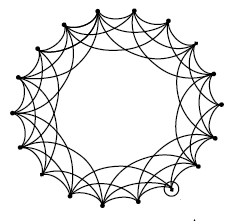
\includegraphics[scale=0.7]{Figures/ring_lattice.png}
    \rule{35em}{0.5pt}
    \caption[A ring lattice]{A ring lattice}
    \label{fig:ring_lattice}
\end{figure}

We initialize the input and output weight matrices as well as the biases using the same process as in the RNN model. 
The parameters of the model for the hessian free optimization step are only the non-zero weights. 

\subsection{Evolution Step}

The evolution step consist of three different steps:
\begin{itemize}
    \item Adding weights: if two consecutive weights ($ab$, $bc$) are above a weight treshold, we diminush them by half and create a new connection ($ac$)
    \item deleting weights that are near zero
    \item Adding neurons: We duplicate with a small noise (on the connections to break the symmetry) the neuron with the highest clustering coefficient. 
\end{itemize}


\subsection{Reordering Step}
    The goal of the reordering step is to switch neurons position in $Whh$ so that the matrix keeps the same shape as in the initialization step. 









